Nesse capítulo, serão apresentados os resultados obtidos utilizando o método multiescala para solução dos sistemas lineares decorrentes do operador apresentado no capítulo \ref{ch:modelagem}. Os resultados são apresentados na seguinte ordem: resultados em casos que a solução analítica é conhecida,
comparacão entre pré-condicionador aditivo contra multiplicativo, comparações do método multiescala como pré-condicionador contra solver multigrid,
 estudo do número de iterações do solver linear com variação da tolerância do solver grosso.



\section{Soluções Analíticas}

Inicialmente, é necessário atestar que o código de elementos finitos está resolvendo corretamente o operador da equação \ref{eq:edp_geomec}. 
Para isso, foi montado teste semelhante ao mostrado em \cite{irina}, teste consiste em encontrar solução para o problema que possui solução analítica de acordo com a equação mostrada em \ref{eq:irinasol} 
em um domínio $L \times W$.


\begin{equation} \label{eq:irinasol}
  \begin{aligned}
  u_x = 10^{-5} sen(\frac{\pi x}{L}) sen(\frac{\pi y}{W})  \\
  u_y = 10^{-5} sen(\frac{\pi (L-x)}{L}) sen(\frac{\pi x}{W})
  \end{aligned}
\end{equation}

Dada essa solução, é possível calcular o operador do lado direito aplicando o operador e obtendo a função $f: R^2 \rightarrow R^2$ apresentada em \ref{eq:irinald}

\begin{equation} \label{eq:irinald}
f(x, y) = 
\left[\begin{matrix}\frac{E \left(- 2 v + \pi^{2} y \left(v - 1\right) \left(y - 2\right) + 1\right) \sin{\left (\pi x \right )}}{\left(v + 1\right) \left(2 v - 1\right)} \\ \frac{\pi E \left(y - 1\right) \cos{\left (\pi x \right )}}{\left(v + 1\right) \left(2 v - 1\right)}\end{matrix}\right]
\end{equation}

Dessa forma, as equações que representam o problema resolvido são apresentadas em \ref{eq:irinaproblem}
\begin{equation}\label{eq:irinaproblem}
    \begin{aligned}
        S^T C S u = f(x, y) \\
        u(x,y) = [0, 0]^T, \text{ em } \Gamma \\
        L = W = 10
    \end{aligned}
\end{equation}


O erro entre a solução calculada pelo método dos elementos finitos pode então ser comparada
com a solução analítica pode ser calculado conforme a equação \ref{eq:erroAnalitico}.

\begin{equation} \label{eq:erroAnalitico}
    \epsilon_{inf} =\frac{|u_{fem} - u_{analitico}|}{|u_{analitico}|}
\end{equation}

onde $u_{analitico} = [u_x(x_0, y_0), u_y(x_1, y_1), ..., u_x(x_{n_n}, y_{n_n})]^T$ e $u_{fem}$ é a solucão obtida com o método dos elementos finitos. Esse erro é mostrado na \ref{fig:SecondOrderTest} onde no eixo x 
está plotado no eixo x o logaritmo do tamanho de cada elemento e no eixo y o logaritmo do erro analítico também mostra uma reta de coeficiente angular $2$ para comparação com um decaimento
quadrático do erro em função do tamanho de cada elemento da malha.

\begin{figure}[!htbp]
    \caption{Comparação entre solução do grid fino e de diferentes grids grossos.}
    \label{fig:SecondOrderTest}
    \centering
    \includegraphics[width=7cm]{chap08/figs/SecondErrorTest.png}
\end{figure}
    
Um segundo caso com resultado analítico é a condição de cisalhamento puro (Simple Shear). 
Nesse caso, o problema é definido na forma apresentada em \ref{eq:simpleshear}. A solução
é dada por $u(x,y) = [y, 0]^T$. Portanto, dado que o a solução é um polinomio do primeiro grau,
essa pode ser representada pelo espaço gerado pelas funções de base bilineares e, então,
os erros de truncamento nesse caso não existem ficando apenas com erros de arredondamento.

\begin{equation}\label{eq:simpleshear}
    \begin{aligned}
        S^T C S u = 0 \\
        u(x,y) = [10^{-6}, 0]^T, \text{ em } \{x, y \in \Gamma | y \neq 1\} \\
        u(x,y) = [10^{-6}y, 0]^T, \text{ em } \{x, y \in \Gamma | x = 0 \text{ ou } x = 1\} \\
        u(x,y) = [0, 0]^T, \text{ em } y=0
    \end{aligned}
\end{equation}

A variação do erro com o tamanho da malha é apresentado na figura \ref{fig:SecondErrorTestSimpleShear} e pode-se observar que
nesse caso o erro relativo menor que $10^{-12}$ que é bem menor que do caso anterior por conta do erro de truncamento ser zero e também
não decai com o tamanho da malha.

\begin{figure}[!htbp]
    \label{fig:SecondErrorTestSimpleShear}
    \centering
    \includegraphics[width=7cm]{chap08/figs/SecondErrorTestSimpleShear.png}
    \caption{Comparação entre solução do grid fino e de diferentes grids grossos.}
\end{figure}

Atestado o bom funcionamento do método dos elementos finitos para solução de problemas com a solução
analítica conhecida, será aplicado agora o método multiescala para verificar o seu correto funcionamento.

\section{Modelos de simulação utilizados}

Os resultados das próximas seções serão apresentados em relação aos modelos apresentados na Tabela \ref{tab:descricaoModelos}. 
A tabela apresenta o tamanho dos grid dos modelos e se são baseados em casos reais ou não.


\begin{table}[]
    \caption{Tabela com os casos que serão apresentados os resultados.}\label{tab:descricaoModelos}
    \centering
    \begin{tabular}{ccccl}
    \cline{1-4}
    \multicolumn{1}{|c|}{\textbf{Nome}} & \multicolumn{1}{c|}{\textbf{Nx}} & \multicolumn{1}{c|}{\textbf{Ny}} & \multicolumn{1}{c|}{\textbf{Caso Real}} &  \\ \cline{1-4}
    \multicolumn{1}{|c|}{caso A}        & \multicolumn{1}{c|}{100}         & \multicolumn{1}{c|}{100}         & \multicolumn{1}{c|}{}                   &  \\ \cline{1-4}
    \multicolumn{1}{|c|}{caso B}        & \multicolumn{1}{c|}{320}         & \multicolumn{1}{c|}{320}         & \multicolumn{1}{c|}{}                   &  \\ \cline{1-4}
    \multicolumn{1}{|c|}{caso C}        & \multicolumn{1}{c|}{103}         & \multicolumn{1}{c|}{56}          & \multicolumn{1}{c|}{}                   &  \\ \cline{1-4}
    \multicolumn{1}{|c|}{caso D}        & \multicolumn{1}{c|}{244}         & \multicolumn{1}{c|}{71}          & \multicolumn{1}{c|}{Sim}                &  \\ \cline{1-4}
    \multicolumn{1}{|c|}{caso E}        & \multicolumn{1}{c|}{582}         & \multicolumn{1}{c|}{336}         & \multicolumn{1}{c|}{Sim}                &  \\ \cline{1-4}
    \multicolumn{1}{l}{}                & \multicolumn{1}{l}{}             & \multicolumn{1}{l}{}             & \multicolumn{1}{l}{}                    &  \\
    \multicolumn{1}{l}{}                & \multicolumn{1}{l}{}             & \multicolumn{1}{l}{}             & \multicolumn{1}{l}{}                    & 
    \end{tabular}
\end{table}


Os casos A e B são baseados nos casos sintéticos apresentados em \cite{casteletto} e \cite{irina}, nesses casos foram utilizados
uma compressibilidade vertical uniaxial $c_M$ desenvolvida em \cite{correlacaoE} apresentada na equação \ref{eq:correlacaoCm}

\begin{equation} \label{eq:correlacaoCm}
    c_M = 0.01241 |\sigma_y^\prime|^{-1.1342}
\end{equation}

onde $c_M$ e $\sigma_y^\prime$ são expressas em [bar$^{-1}$] e [bar] e  $\sigma_y^\prime$ representa a tensão vertical efetiva.
Considerando um gradiente de pressão de 0.1 bar/m e coeficiente de biot igual a um a tensão efetiva total pode ser calculada de acordo com \ref{eq:correlacaoTensao}.




\begin{equation} \label{eq:correlacaoTensao}
\sigma_y^\prime = \sigma_y + p = -0.12218|y| + 0.1 |y|
\end{equation}

E o módulo de Young pode ser calculado em função apenas da profundidade equação substituindo os valores de \ref{eq:correlacaoCm} e \ref{eq:correlacaoTensao} em \ref{eq:correlacaoYoung}.

\begin{equation} \label{eq:correlacaoYoung}
    E = \frac{(1-2\poisson)(1+\poisson)}{(1-\poisson)c_M}
\end{equation}

O grid utilizado é apresentado \ref{fig:gridBase10x10}, esse grid teve cada uma das células divididas em com 10 cortes verticais e 
10 cortes horizontais igualmente espassados para gerar um o caso A e de forma análoga dividida em 32 cortes horizontais e 
32 cortes verticais para gerar o caso B.

\begin{figure}[!htbp]
    \label{fig:gridBase10x10}
    \centering
    \includegraphics[height=4cm]{interrogacao.png}
    \caption{Grid base utilizado para construção dos casos A e B.}
\end{figure}

o caso C é um caso de reservatório sintético com grid de geometria mais próxima aos reservatórios reais, além disso, diferentemente dos casos A e B os valores
de poisson não são constantes ao longo do domínio. A figura \ref{fig:casoCgrid} apresenta o grid e os valores do módulo de Young e módulo de Poisson.
São apresentados também figuras dos casos D e E que tiveram as escalas omitidas por se tratarem de modelos de campos reais.


\begin{figure}[!htbp]
    \label{fig:casoCgrid}
    \centering
    \includegraphics[height=4cm]{interrogacao.png}
    \caption{Propriedades (módulo de Young e coeficiente de poisson) para caso C }
\end{figure}


\begin{figure}[!htbp]
    \label{fig:casoDgrid}
    \centering
    \includegraphics[height=4cm]{interrogacao.png}
    \caption{Propriedades (módulo de Young e coeficiente de poisson) para caso D }
\end{figure}

\begin{figure}[!htbp]
    \caption{Propriedades (módulo de Young e coeficiente de poisson) para caso D }
    \label{fig:casoEgrid}
    \centering
    \includegraphics[height=4cm]{interrogacao.png}
\end{figure}


As condições de contorno utilizadas são representadas na figura \ref{fig:CondicoesContorno}. 

\begin{figure}[!htbp]
    \caption{Esquema das condições de contorno das simulações. Borda inferior com deslocamentos nulos, bordas laterais com deslocamentos em y permitidos e borda superior livre.}
    \label{fig:CondicoesContorno}
    \centering
    \includegraphics[height=4cm]{chap08/figs/CondicoesContorno.png}
\end{figure}


\section{Método Multiescala como pré-condicionador}

\subsection{Comparação entre pré-condicionadores aditivos e multiplicativos}
O trabalho \cite{casteletto} apresenta a utilização do pré-condicionador multiescala ($M_{ms}$) em conjunto com o um pré-condicionador ($M_h$) no grid fino de forma multiplicativa. 
Essa combinação visa reduzir os erros de alta frequência através do $M_h$ enquanto os erros de baixa frequencia são eliminados pelo pré-condicionador multiescala. 
O acoplamento multiplicativo tem a desvantagem de precisar de uma multiplicação matriz vetor além da aplicação dos pré-condicionadores
e, portanto, o número de iterações tem que ser reduzido o suficiente para compensar todas essas operações. Um alternativa é aplicação
dos pré-condicionadores de forma aditiva, pois, nesse caso, não é necessária a multiplicação matriz vetor adicional. Outra vantagem do operador
aditivo é que caso os dois pré-condicionadores sejam simétricos o pré-condicionador conjunto também é simétrico e pode ser utilizado juntamente
com o gradiente conjugado para a solução dos sistemas lineares.


Os testes as seguir mostram o número de iterações do bicgstab utilizando pré-condicionadores multiplicativos e aditivos do caso A e caso B utilizados para comparação
com o método Bicgstab dado que o pré-condicionador multiplicativo não necessariamente é simétrico. Nesses testes o pré-condicionador $M_h$ utilizado foi o ILU(0).

As tabelas \ref{table:precondcasoAcomp} e \ref{table:precondcasoBcomp} mostram a quantidade de iterações e os respectivos resíduos feita pelos pré-condicionadores aplicados a solução do sistema. 

É importante notar que a quantidade de iterações é bem próxima, mostrando que a quantidade
nos problemas apresentados é melhor utilizar o pré-condicionador aditivo em relação ao pré-condicionador multiplicativo. Dessa forma, os próximos
testes serão feito utilizando com o solver o Gradiente Conjugado.

\begin{table}[]
    \caption{Comparação de pré-condicionador aditivo contra multiplicativo para caso A utilizando como solver linear o método Bicgstab para diferentes níveis de engrossamento do nível grosso.}
    \label{table:precondcasoAcomp}
    \begin{tabular}{c|c|l|c|l|}

    \cline{2-5}
                                          & \multicolumn{4}{c|}{Pré-condicionador}                                                        \\ \cline{2-5} 
                                          & \multicolumn{2}{c|}{$\preconmult$}               & \multicolumn{2}{c|}{$\preconadd$}                \\ \hline
    \multicolumn{1}{|c|}{Elemento Grosso} & Iterações & \multicolumn{1}{c|}{Resíduo}      & Iterações & \multicolumn{1}{c|}{Resíduo}      \\ \hline
    \multicolumn{1}{|c|}{2x2}             & 7         & \multicolumn{1}{c|}{1.038308e-11} & 9         & \multicolumn{1}{c|}{8.186640e-12} \\ \hline
    \multicolumn{1}{|c|}{5x5}             & 16        & 1.720391e-11                      & 17        & 2.063517e-11                      \\ \hline
    \multicolumn{1}{|c|}{10x10}           & 25        & 1.872316e-11                      & 28        & 5.663356e-12                      \\ \hline
    \multicolumn{1}{|c|}{20x20}           & 38        & 1.643261e-11                      & 38        & 2.842643e-11                      \\ \hline
    \end{tabular}
\end{table}


\begin{table}[]
    \caption{Comparação de pré-condicionador aditivo contra multiplicativo para caso B utilizando como solver linear o método Bicgstab para diferentes níveis de engrossamento do nível grosso.}
    \label{table:precondcasoBcomp}
    \begin{tabular}{c|c|l|c|l|}
    \cline{2-5}
                                          & \multicolumn{4}{c|}{Pré-condicionador}                                                        \\ \cline{2-5} 
                                          & \multicolumn{2}{c|}{$\preconmult$}               & \multicolumn{2}{c|}{$\preconadd$}                \\ \hline
    \multicolumn{1}{|c|}{Elemento Grosso} & Iterações & \multicolumn{1}{c|}{Resíduo}      & Iterações & \multicolumn{1}{c|}{Resíduo}      \\ \hline
    \multicolumn{1}{|c|}{32x32}           & 86        & \multicolumn{1}{c|}{4.352864e-11} & 80        & \multicolumn{1}{c|}{4.187004e-11} \\ \hline
    \multicolumn{1}{|c|}{64x64}           & 126       & 4.645286e-11                      & 119       & 2.214093e-11                      \\ \hline
    \multicolumn{1}{|c|}{80x80}           & 133       & 4.939883e-11                      & 135       & 3.432757e-11                      \\ \hline
    \end{tabular}
\end{table}


\subsection{Comparação com Multigrid}

Nessa seção, são apresentadas comparações entre o método multiescala e o método multigrid. Para esse comparação foi utilizado o solver multigrid Pyamg, que é um solver multigrid  descrito e implementado em \cite{OlSc2018}. 
Dado a grande quantidade de parâmetros necessários para a configuração dos solver multigrid como: a quantidade de níveis devem ser utilizados, quantidade de relaxações em cada nível, qual o tipo de relaxação será utilizada, dentre outras variáveis, foi utilizado o script solver\_diagnotics.py disponibilizado pela equipe do Pyamg no repositório ( https://github.com/pyamg/pyamg-examples ). Esse script testa diferentes configurações de solver multigrid para uma dada matriz e seleciona aquele mais eficiente para o problema proposto.

Os resultados para cada uma das matrizes mostrou um solver comum a todas as matrizes que possuia os seguintes parâmetros:

\begin{itemize}
    \item máximo de quinze níveis multigrid
    \item relaxação "Block Gauss Seidel Sweep" 
    \item ciclos V
    \item multigrid como pré-condicionador para o Gradiente Conjugado
\end{itemize}

A figura \ref{fig:reservatorio100x100_1} apresenta o tempo de solução do sistema utilizando o método multiescala e multigrid (Pyamg) como precondicionador para o gradiente conjugado para o caso A. São apresentados o resíduo ao longo das iterações, o tempo de execução do solver, a quantidade de iterações do solver linear e o tempo da iteração.

\begin{figure}[!htbp]
\caption{Resultados para caso A. À esquerda Histórico do resíduo relativo ao longo das iterações. 
Ao centro, tempo do solver em segundos. À direita o tempo do solver por iteração. }
\label{fig:reservatorio100x100_1}
\centering
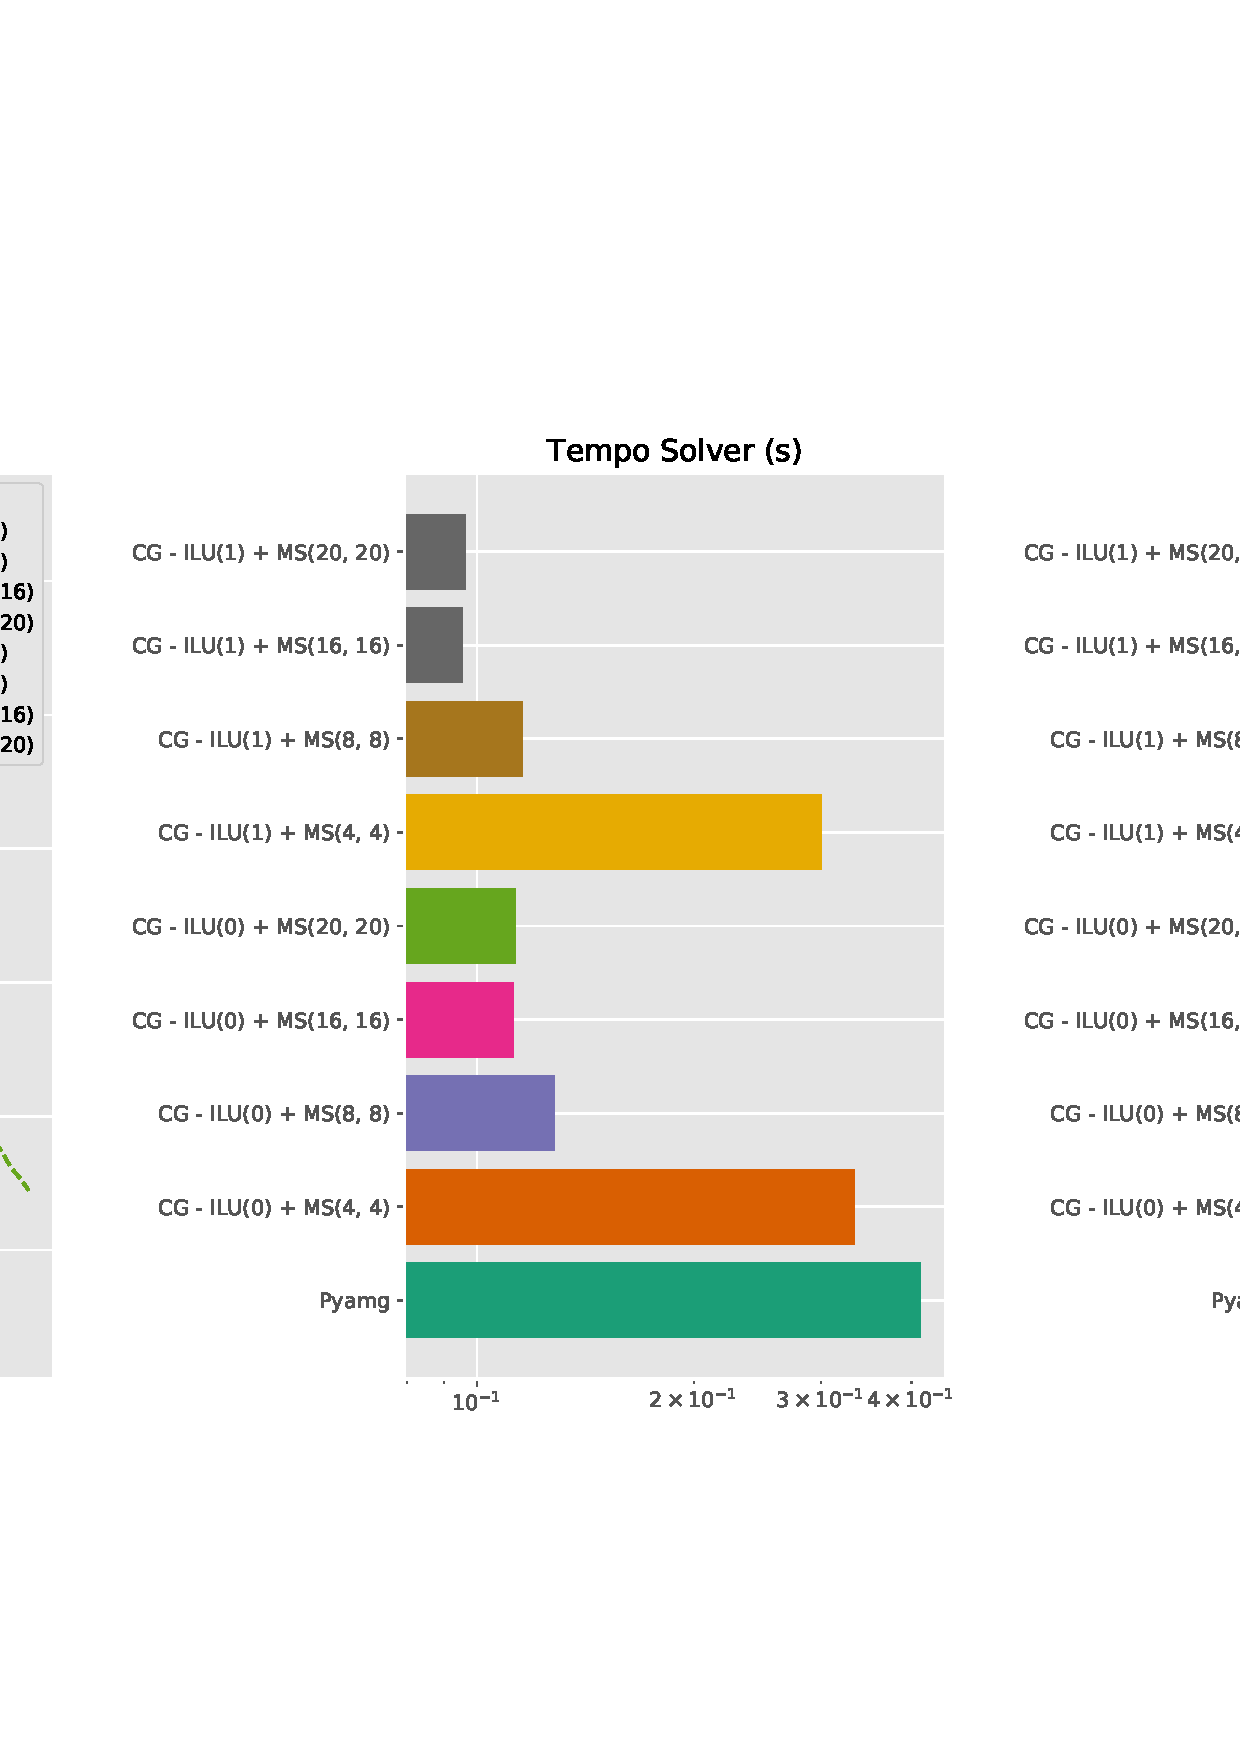
\includegraphics[width=\textwidth]{chap08/figs/reservatorio100x100_1.png}
\end{figure}

Um primeiro ponto a se observar no gráfico da esquerda é o aumento do número de iterações a cada vez que se aumenta o fator de engrossamento da malha. 
Isso ocorre pois a solução do problema grosso se torna cada vez mais distante da solução da malha fina fazendo com que o pré-condicionador funcione pior. 
Entretanto, quanto mais grossa a malha, mais fácil a solução sistema linear grosso e, portanto, existe uma solução de compromisso 
entre o engrossamento da malha e o tempo de execução. É importante lembrar também que sempre é necessário pagar o custo da multiplicação pelo
operador de prolongamento e de restrição que independe do nível de engrossamento, por conta disso, o tempo da iteração do engrossamento 16x16
é semelhante ao 20x20. No caso A, a solução de menor tempo é quando o nível grosso é construído ao se montar elementos grossos utilizando 16x16 elementos finos. 



Na figura \ref{fig:reservatorio100x100_2} é apresentado a comparação da solução do sistema utilizando o melhor método multiescala com o gradiente conjugado 
utilizando como precondicionador o ILU(0), ILU(1) e solver multigrid Pyamg. 
ode-se notar que apesar da redução de iterações dos método multiescala e do método multigrid, os pré-condicionadores ILU(0) e ILU(1) são mais eficientes na resolução do sistema. 


\begin{figure}[!htbp]
\caption{Resultados para caso A. Histórico do resíduo relativo ao longo das iterações, tempo do solver em segundos, número de iterações em função do fator de engrossamento da malha e tempo do solver por iteração. }
\label{fig:reservatorio100x100_2}
\centering
\includegraphics[width=\textwidth]{chap08/figs/reservatorio100x100_2.png}
\end{figure}


As figuras \ref{fig:reservatorio320x320_1} e \ref{fig:reservatorio320x320_2} apresentam os mesmos resultados para o caso B.
Nesse caso, o engrossamento multiescala de 20x20 é o que resolve o solver em menor tempo, conseguindo inclusive superar o tempo de solução com o solver pré-condicionador ILU(1).
O tempo de solução com MS+ILU(1) tem uma melhora de 11,4\% em relação ao tempo do ILU(0). Quando comparado MS+ILU(1) contra ILU(1) o tempo de execução é 45,7\% tempo menor.
Além disso, o Pyamg não conseguiu convergir para a solução do problema, parando a execução quando o resíduo atingiu a casa dos $10^{-3}$


\begin{figure}[!htbp]
\caption{Resultados para caso B. Histórico do resíduo relativo ao longo das iterações, tempo do solver em segundos, número de iterações em função do fator de engrossamento da malha e tempo do solver por iteração. }
\label{fig:reservatorio320x320_1}
\centering
\includegraphics[width=\textwidth]{chap08/figs/reservatorio320x320_1.png}
\end{figure}


\begin{figure}[!htbp]
\caption{Resultados para caso B. Histórico do resíduo relativo ao longo das iterações, tempo do solver em segundos, número de iterações em função do fator de engrossamento da malha e tempo do solver por iteração. }
\label{fig:reservatorio320x320_2}
\centering
\includegraphics[width=\textwidth]{chap08/figs/reservatorio320x320_2.png}
\end{figure}


A seguir são apresentados resultados para o corte dos modelos D e E respectivamente nas figuras \ref{fig:casoD_2} e \ref{fig:casoE_2}. 
São apresentadas apenas a comparação entre os pré-condicionadores multiescala, Pyamg, ILU(0) e ILU(1). 


A seguir, as figuras \ref{fig:casoC_2}, \ref{fig:casoD_2} e \ref{fig:casoE_2} apresentam os resultados para os casos C, D e E. 
Em todos os gráficos é mostrado apenas o pré-condicionador multiescala que obteve o melhor desempenho entre os fatores de engrossamento de 2x2, 4x4, 8x8, 16x16, 32x32.


% \begin{figure}[!htbp]
% \label{fig:casoD_1}
% \centering
% \includegraphics[width=\textwidth]{chap08/figs/casoD_1.png}
% \caption{Resultados para caso D. Histórico do resíduo relativo ao longo das iterações, tempo do solver em segundos, número de iterações em função do fator de engrossamento da malha e tempo do solver por iteração. }
% \end{figure}

\begin{figure}[!htbp]
\caption{Comparação entre multiescala, multigrid e pré-condicionador ILU para o caso D. Histórico do resíduo relativo ao longo das iterações, tempo do solver em segundos e tempo do solver por iteração. }
\label{fig:casoD_2}
\centering
\includegraphics[width=\textwidth]{chap08/figs/casoD_2.png}
\end{figure}

    
\begin{figure}[!htbp]
\caption{Comparação entre multiescala, multigrid e pré-condicionador ILU para o caso D. Histórico do resíduo relativo ao longo das iterações, tempo do solver em segundos e tempo do solver por iteração. }
\label{fig:casoE_2}
\centering
\includegraphics[width=\textwidth]{chap08/figs/casoE_2.png}
\end{figure}


\subsection{Acurácia da solução grossa}

Nos resultados mostrados nas seções anteriores, era utilizado um solver direto para resolver 
o sistema grosso. Em casos que a malha foi suficientemente reduzida esse tempo de solução é desprezível,
porém, para casos o fator de engrossamento é pequeno resolver exatamente o nível grosso aumenta
o tempo de execução (por exemplo, o caso ILU(1) + MS(4,4) em \ref{fig:reservatorio100x100_1}). 
Além disso, caso modelos muito refinados sejam utilizados o espaço grosseiro pode continuar
grande e precise ser resolvido com métodos iterativos, como por exemplo para soluções de casos
com centenas de milhões de elementos como o mostrado em \cite{geomecrio}.


A avaliação foi feita da seguinte maneira: foi avaliada a quantidade de iterações para resolver o sistema linear com tolerância de $10{-6}$ utilizando o pré-condicionador multiescala com solver do espaço grosso um gradiente conjugado com tolerância variando de $10^{-10}$  a $10^{-1}$. 